\chapter{IPsec}

\section{VPN}

A VPN is a private network that is created over a public network, usually the Internet. A VPN is virtual because it carries information within a private network, but that information is actually transported over a public network. A VPN is private in that the traffic is encrypted to keep the data confidential while it is transported across the public network.\\

A remote-access VPN is not statically set up, but instead allows for dynamically creating, changing, and terminating connection. Using remote-access VPN, remote host has to install a special VPN software. A site-to-site VPN is statically set up and always active even if network communication is terminated. Site-to-site VPN is transparent to internal hosts.\\

There are two kinds of VPN topology: Hairpinning and Split tunneling. Hairpinning allows VPN traffic received on a single interface to be routed back out that same interface. Split tunneling allows traffic that originates from a remote-access client to be split according to traffic that must cross a VPN and traffic that is destined for the public Internet. 

\section{IPsec protocols}

IPsec is a layer-3 VPN technology which is often used for site-to-site VPN. The IPsec framework uses various protocols and algorithms:

\begin{itemize}
\item IPsec protocol: AH, ESP, AH+ESP
\item Confidentiality (encryption): DES, 3DES, AES, SEAL
\item Integrity (hash): MD5, SHA
\item Authentication: PSK, RSA
\item Key exchange: DH family
\end{itemize}

\textbf{Authentication Header (AH)} is IP protocol 51 and does not provide data confidentiality because the data payload is not encrypted. However, AH achieves authenticity applying a keyed one-way hash function (MD5 or SHA) to the packet. The AH function is applied to the entire packet, except for any IP header fields that normally change in transit. That is why AH will not work with NAT.\\

\textbf{Encapsulating Security Payload (ESP)} is IP protocol 50 and provides data confidentiality, integrity, and authentication. ESP encrypts entire original IP datagram and ESP trailer. Optionally, ESP can also enforce anti-replay protection, which verifies that each packet is unique and is not duplicated. This protection ensures that a hacker cannot intercept packets and insert changed packets into the data stream.\\

ESP and AH can be applied to IP packets in two different modes, transport mode and tunnel mode. In transport mode, security is provided only for the transport layer of the OSI model and above. Transport mode protects the payload of the packet but not IP address. Tunnel mode provides security for the complete original IP packet. The original IP packet is encrypted and then it is encapsulated in another IP packet. This is known as IP-in-IP encryption. \\

The Internet Key Exchange (IKE) is a key management protocol, which negotiates IPsec security associations (SAs) and enables IPsec secure communications. IKE uses \textbf{UDP port 500} to implement key exchange protocols inside the Internet Security Association Key Management Protocol (ISAKMP) framework\footnote{ISAKMP defines the message format, key exchange mechanism, and the negotiation process for IPsec.}. Instead of transmitting keys directly across a network, IKE calculates shared keys based on the exchange of a series of data packets. 

\section{Operation}

IPsec negotiation to establish a VPN involves five steps, which include IKE Phase 1 and Phase 2:

\begin{enumerate}
\item \textbf{ISAKMP tunnel:}  When host A sends ``interesting'' traffic to host B, an ISAKMP tunnel is initiated. Traffic is considered interesting when it travels between the peers and meets the criteria that are defined in an ACL.

\item \textbf{IKE Phase 1:} The peers negotiate the ISAKMP policy. When the peers agree on the policy and are authenticated, a secure tunnel is created.

\item \textbf{IKE Phase 2:} The peers negotiate the IPsec policy using the tunnel in phase 1. In this phase, a separate key exchange is required for each data flow.

\item The IPsec tunnel is created.

\item The IPsec tunnel terminates manually by the user, or when their lifetime expires.
\end{enumerate}

\section{Site-to-site VPN using IPsec configuration}

\begin{figure}[hbtp]
\caption{Site-to-site VPN topology}\label{VPNtopolgy}
\centering
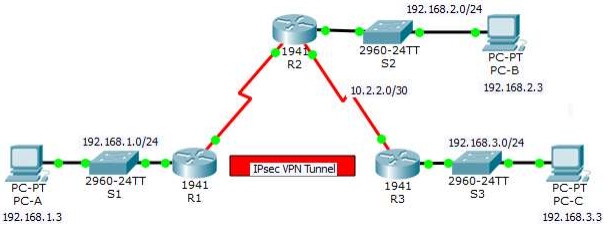
\includegraphics[scale=0.8]{pictures/VPNtopolgy.PNG}
\end{figure}


\begin{figure}[hbtp]
\caption{Adressing table}\label{AddressTable}
\centering
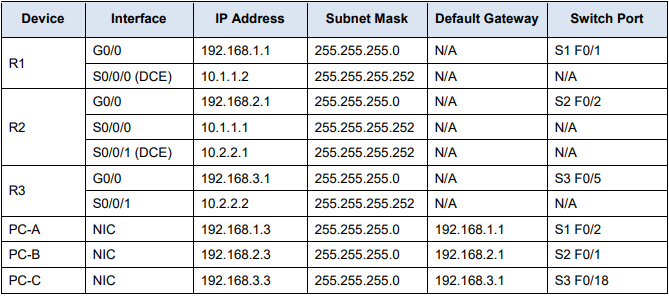
\includegraphics[scale=0.8]{pictures/AddressTable.PNG}
\end{figure}


The configuration tasks for the topology in figure \ref{VPNtopolgy} and addressing table in figure \ref{AddressTable} are shown in order as below:

\begin{enumerate}
\item Enable the Security Technology package and ISAKMP

\item Identify interesting traffic: Configure ACL to permit the traffic from the R1-LAN to R3-LAN. Whenever this traffic is active, VPN is triggered.

\item ISAKMP policy: Use the mnemonic \textbf{HAGLE} to remember the five SAs to configure: Hash, Authentication, Group, Lifetime, and Encryption. Note that the address of the peer router R3 is the address of serial interface connected to the Internet (s0/0/0).

\item Transform set: This step is to configure the set of encryption and hashing algorithms that will be used to transform the data sent through the IPsec tunnel. This is called the transform set. In this situation, we create a transform set named VPN-SET that uses an ESP transform with an AES 256 for encryption and SHA for hash. The transform sets on R1 and R3 must match. 

\item Create a crypto map VPN-MAP to bind all policy parameters together. Use sequence number 10 and identify it as an ipsec-isakmp map. In the following commands,the perfect forwarding secrecy type is set using the \code{set pfs} command.

\item Configure the crypto map on the outgoing interface.

\item Repeat the above steps on R3.
\end{enumerate}

\begin{sexylisting}{Site-to-site IPsec}
#ENABLE SECURITY FEATURE
license boot module c1900 technology-package securityk9
crypto isakmp enable

#INTERESTING TRAFFIC
access-list 110 permit ip 192.168.1.0 0.0.0.255 192.168.3.0 0.0.0.255

#ISAKMP POLICY
crypto isakmp policy 10
	hash sha 
	authentication pre-share
	group 14
	lifetime 3600
	encryption aes 256
	exit
crypto isakmp key vpnpa55 address 10.2.2.2	

#TRANSFORM SET
crypto ipsec transform-set VPN-SET esp-aes esp-sha-hmac

#CRYPTO MAP
crypto map VPN-MAP 10 ipsec-isakmp
	description VPN connection to R3
	set peer 10.2.2.2
	set transform-set VPN-SET
	set pfs group14
	set security-association lifetime seconds 900 
	match address 110
	exit

#APPLY TO INTERFACE
interface s0/0/0
	crypto map VPN-MAP
	exit

#VERIFICATION
show crypto ipsec transform-set 
show crypto map
show crypto isakmp sa
show crypto ipsec sa		
\end{sexylisting}
